% ***********************************************************
% ******************* PHYSICS HEADER ************************
% ***********************************************************
% Version 2
\documentclass[11pt]{article}
\usepackage{amsmath} % AMS Math Package
\usepackage{amsthm} % Theorem Formatting
\usepackage{amssymb}	% Math symbols such as \mathbb
\usepackage{graphicx} % Allows for eps images
\usepackage{multicol} % Allows for multiple columns
\usepackage[dvips,letterpaper,margin=0.75in,bottom=0.5in]{geometry}
\usepackage{authblk} % Allows for authors from multiiple institutes
\renewcommand\Authands{ and } % for authblk
\usepackage{indentfirst} % to have indent for the 1st paragraph of each section

 % Sets margins and page size
\pagestyle{empty} % Removes page numbers

\makeatletter % Need for anything that contains an @ command

\newcommand{\affil}[1]{\def\@affilname{#1}}
\def\@affil{\@affilname}

\renewcommand{\maketitle} % Redefine maketitle to conserve space
{ \begingroup \vskip 10pt \begin{center} \large {\textbf{\@title}}
\vskip 10pt \large \@author \vskip 10pt \large \@affil \end{center}
\vskip 10pt \endgroup \setcounter{footnote}{0} }

\makeatother % End of region containing @ commands
\renewcommand{\labelenumi}{(\alph{enumi})} % Use letters for enumerate
% \DeclareMathOperator{\Sample}{Sample}
\let\vaccent=\v % rename builtin command \v{} to \vaccent{}
\renewcommand{\v}[1]{\ensuremath{\mathbf{#1}}} % for vectors
\newcommand{\gv}[1]{\ensuremath{\mbox{\boldmath$ #1 $}}}
% for vectors of Greek letters
\newcommand{\uv}[1]{\ensuremath{\mathbf{\hat{#1}}}} % for unit vector
\newcommand{\abs}[1]{\left| #1 \right|} % for absolute value
\newcommand{\avg}[1]{\left< #1 \right>} % for average
\let\underdot=\d % rename builtin command \d{} to \underdot{}
\renewcommand{\d}[2]{\frac{d #1}{d #2}} % for derivatives
\newcommand{\dd}[2]{\frac{d^2 #1}{d #2^2}} % for double derivatives
\newcommand{\pd}[2]{\frac{\partial #1}{\partial #2}}
% for partial derivatives
\newcommand{\pdd}[2]{\frac{\partial^2 #1}{\partial #2^2}}
% for double partial derivatives
\newcommand{\pdc}[3]{\left( \frac{\partial #1}{\partial #2}
 \right)_{#3}} % for thermodynamic partial derivatives
\newcommand{\ket}[1]{\left| #1 \right>} % for Dirac bras
\newcommand{\bra}[1]{\left< #1 \right|} % for Dirac kets
\newcommand{\braket}[2]{\left< #1 \vphantom{#2} \right|
 \left. #2 \vphantom{#1} \right>} % for Dirac brackets
\newcommand{\matrixel}[3]{\left< #1 \vphantom{#2#3} \right|
 #2 \left| #3 \vphantom{#1#2} \right>} % for Dirac matrix elements
\newcommand{\grad}[1]{\gv{\nabla} #1} % for gradient
\let\divsymb=\div % rename builtin command \div to \divsymb
\renewcommand{\div}[1]{\gv{\nabla} \cdot #1} % for divergence
\newcommand{\curl}[1]{\gv{\nabla} \times #1} % for curl
\let\baraccent=\= % rename builtin command \= to \baraccent
\renewcommand{\=}[1]{\stackrel{#1}{=}} % for putting numbers above =
\newtheorem{prop}{Proposition}
\newtheorem{thm}{Theorem}[section]
\newtheorem{lem}[thm]{Lemma}
\theoremstyle{definition}
\newtheorem{dfn}{Definition}
\theoremstyle{remark}
\newtheorem*{rmk}{Remark}

\usepackage[english]{babel}
\graphicspath{{images/}}
\usepackage{siunitx}
\usepackage{lineno}

\def\lycoris{\textsc{Lycoris }}%
\def\GeV{\ifmode {\mathrm{\ Ge\kern -0.1em V }}\else
								 {\textrm{Ge\kern -0.1em V }}\fi}%

% ***********************************************************
% ********************** END HEADER *************************
% ***********************************************************


\begin{document}

\title{{Development of a large active area beam telescope based on the SiD micro-strip sensor}}
\author[3]{Martin Breidenbach}
\author[3]{Dietrich R. Freytag}
\author[3]{Ryan T. Herbst}
\author[1]{Uwe Kraemer}
\author[3]{Benjamin A. Reese}
\author[2,1]{Sebastiaan Roelofs}
\author[1]{Marcel Stanitzki}
\author[1]{Mengqing Wu} % speaker
\affil[1]{\footnotesize Deutsches Elektronen-Synchrotron DESY, Notkestr. 85, 22607 Hamburg, Germany}
\affil[2]{\footnotesize The Hague University of Applied Sciences, Rotterdamseweg 137, 2628 AL Delft, The Netherlands}
\affil[3]{\footnotesize Stanford Linear Accelerator Center SLAC, 2575 Sand Hill Road, Menlo Park, CA 94025 USA}
\maketitle

% \begin{abstract}
% %\linenumbers
%
% A new beam telescope, \lycoris, is currently being installed
% as an improvement for the DESY test beam infrastructure within the EU Horizon2020 AIDA-2020 project~\cite{aida2020}.
% \lycoris telescope is designed to cover a large area for providing a reference momentum measurement to beam users in an \SI{1}{\tesla} solenoid magnet.
% It consists of six layers of the 10$\times$\SI{10}{\square\centi\metre} surface,
% \SI{25}{\micro\metre}(\SI{50}{\micro\metre}) sensor(readout) pitch, single-sided silicon strip sensor,
% giving a spatial resolution better than \SI{10}{\micro\metre} along the bending direction.
% The micro-strip sensor is designed for the SiD tracker, readout by two bump-bonded, KPiX ASICs~\cite{kpix},
% which digitizes and serializes signals from all connected strips, then sends out via one single wirebonded data trace.
% This hybrid-less arrangement enbales \lycoris to accomodate 3 layers of the hybrid-less SiD sensor in \SI{3.2}{\centi\metre} space.
% The presentation will first introduce the telescope with its components,
% then characterization results of the sensor modules will be given based on the beam tests in August and September 2018.
% At the end, the first beam test results of the \lycoris telescope prototype will be shown with a comparison to the simulation.
% \end{abstract}

\subsection*{Brief overview}
%\linenumbers

A large coverage area telescope, namely \textsc{Lycoris}, is currently being installed at the DESY II test beam facility~\cite{desytbf}.
using six layers of the SiD hybrid-less single-sided micro-strip sensor.
\lycoris is designed to address the user demands of reference momentum measurement in an \SI{1}{\tesla} solenoid.
This requires the spatial resolution along the bending direction better than \SI{10}{\micro\metre},
and an active area of 10$\times$\SI{10}{\square\centi\metre} to cover 90\% to 96\% of the beam particles with energies from 1 to \SI{6}{\GeV},
%considering momentum smearing after the magnet wall.
%considering scattering before the last layer.

The micro-strip sensor, see Fig.~\ref{fig:1figs}(left),
is 10$\times$\SI{10}{\square\centi\metre}, \SI{320}{\milli\metre} thick, \SI{25}{\micro\metre}(\SI{50}{\micro\metre}) sensor(readout) pitch.
\lycoris is the first application of this sensor, which was originally designed for the SiD Detector Concept for the ILC~\cite{ILC-2013TDR:det}.
The concept of \lycoris is shown in Fig.~\ref{fig:1figs}(center),
that 6 sensor planes with a \SI{2}{\degree} tilt, build up a 3-D track of the incident particle.
The sensor orientation was studied for an optimized performance with a fixed inter-plane distance.


\begin{figure}[!ht]%
\centering
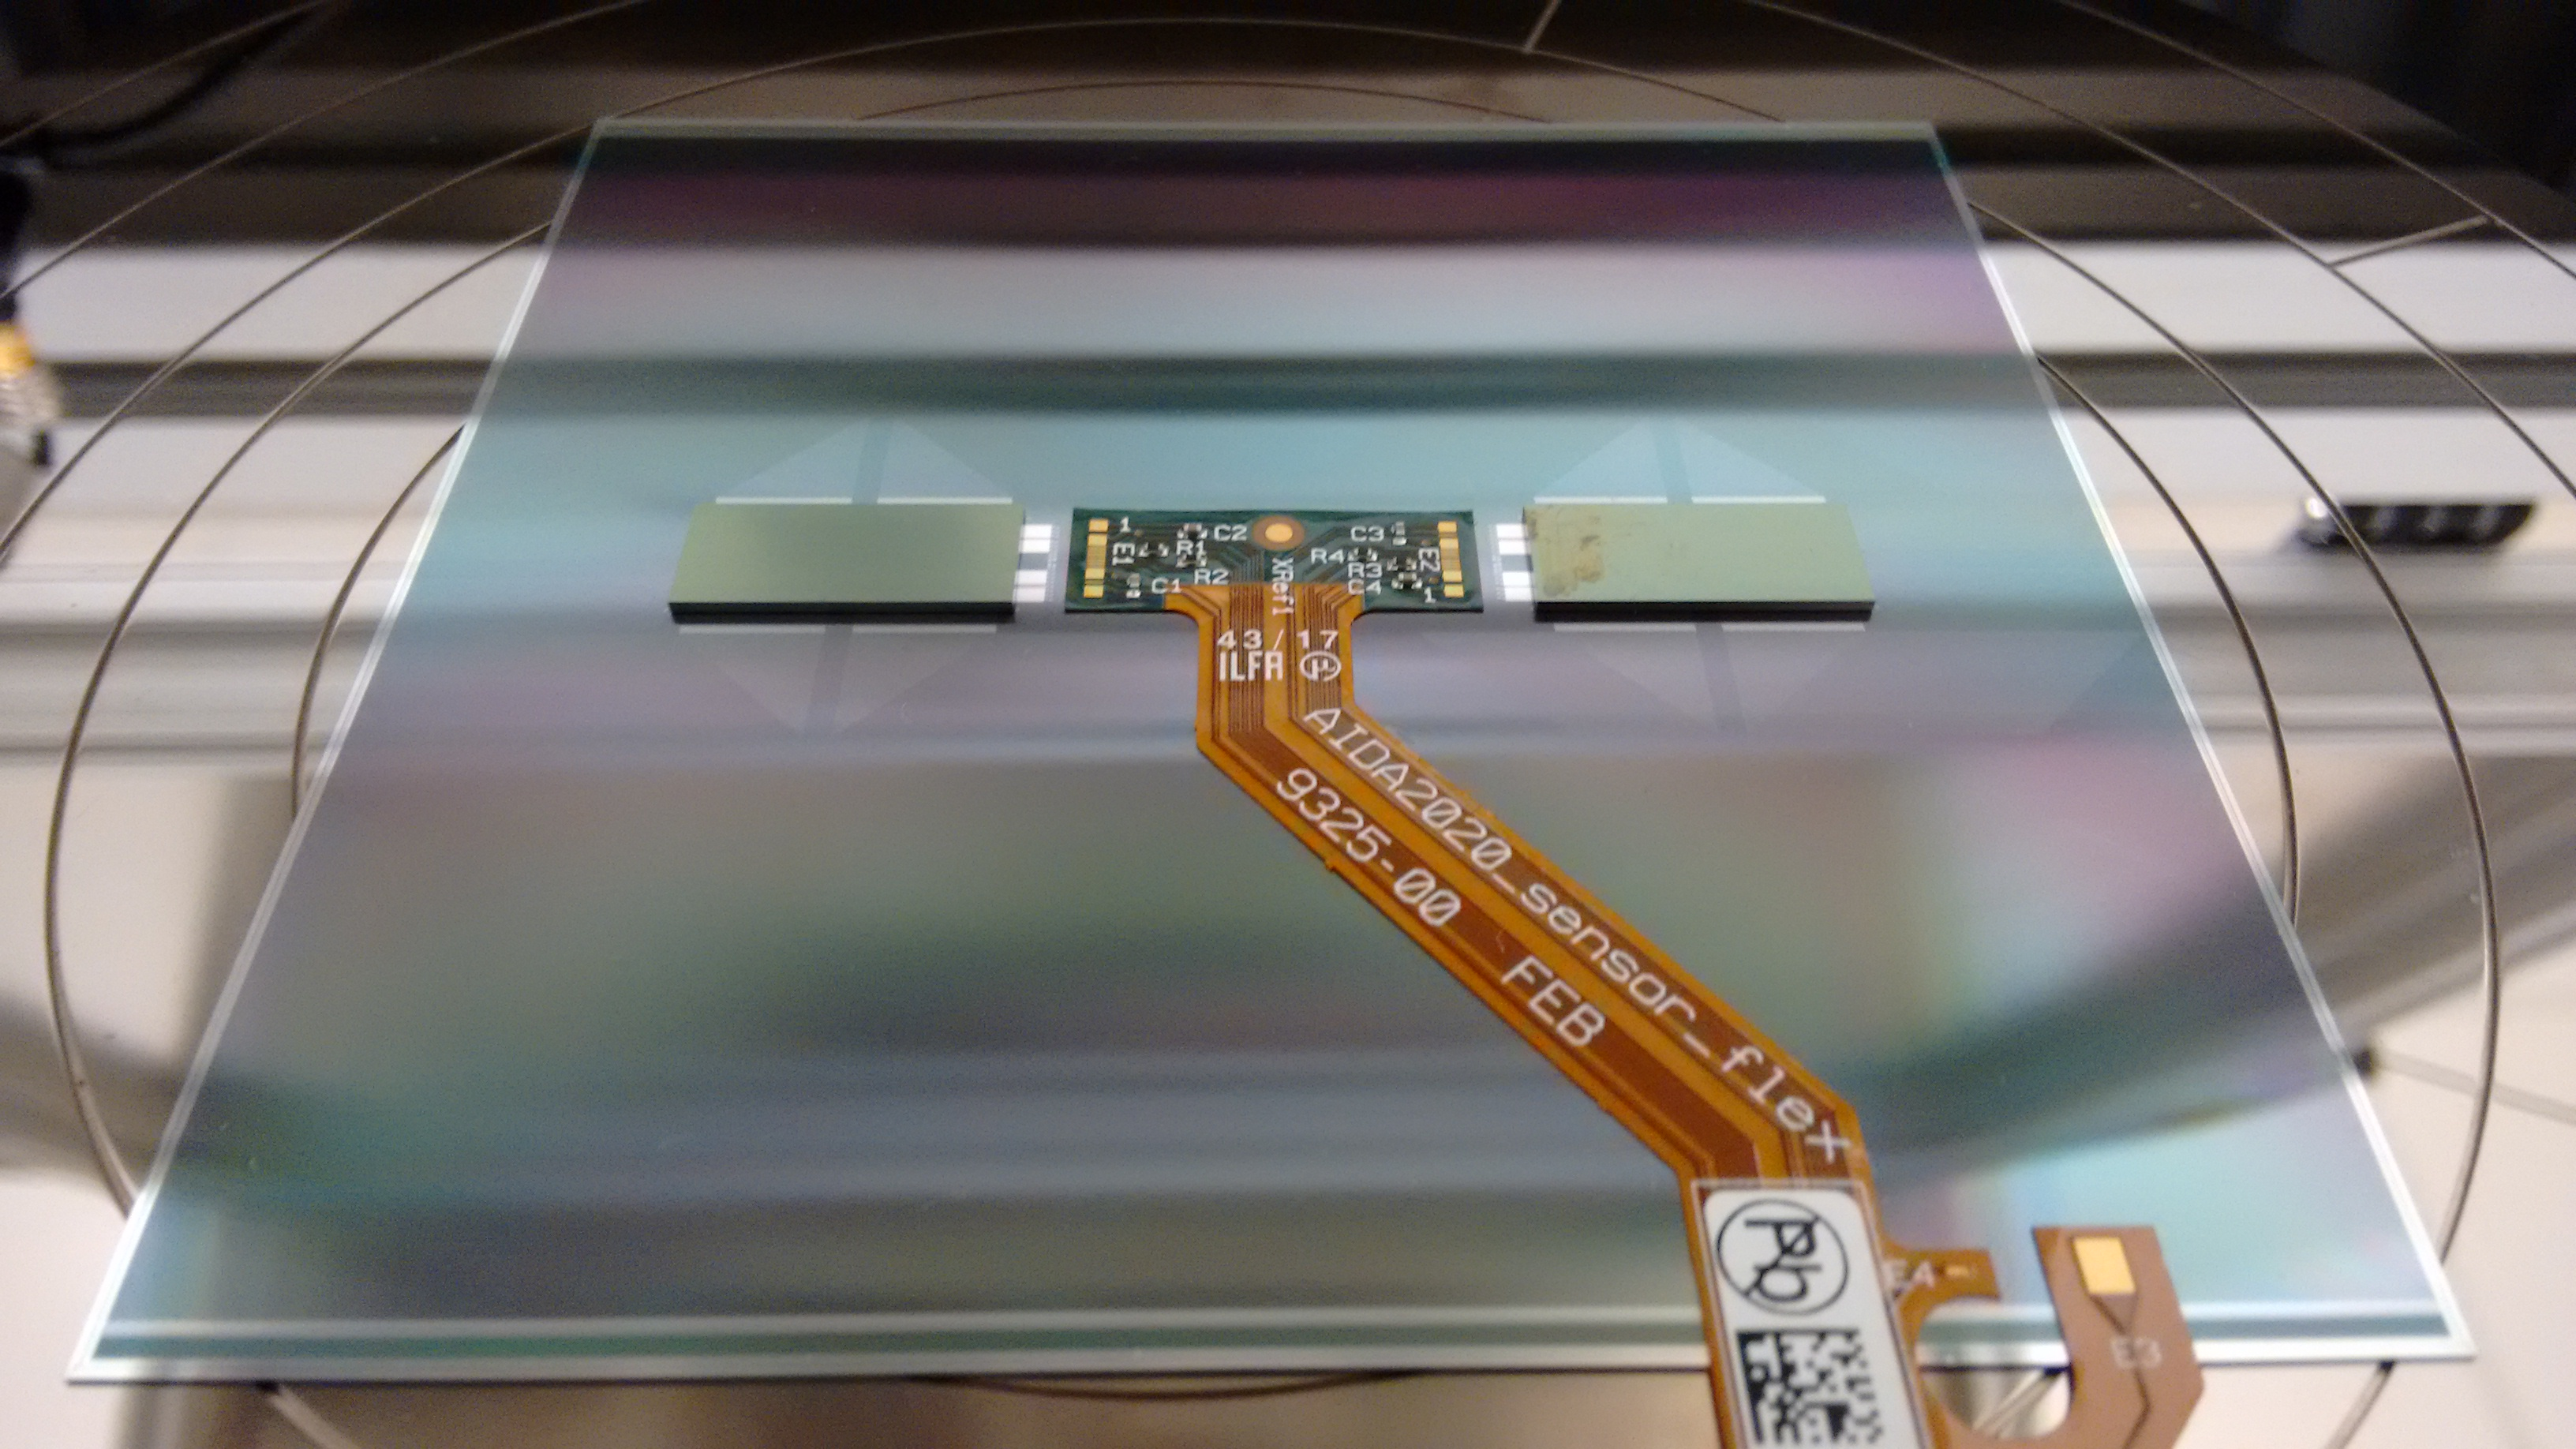
\includegraphics[width=0.33\linewidth]{pics/sensor_module1.jpg}%
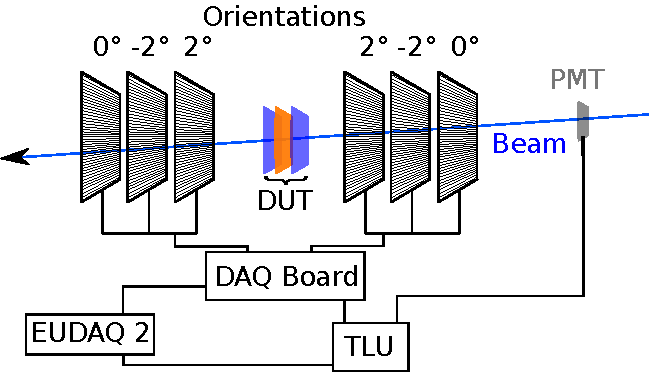
\includegraphics[width=0.33\linewidth]{pics/principle.pdf}%
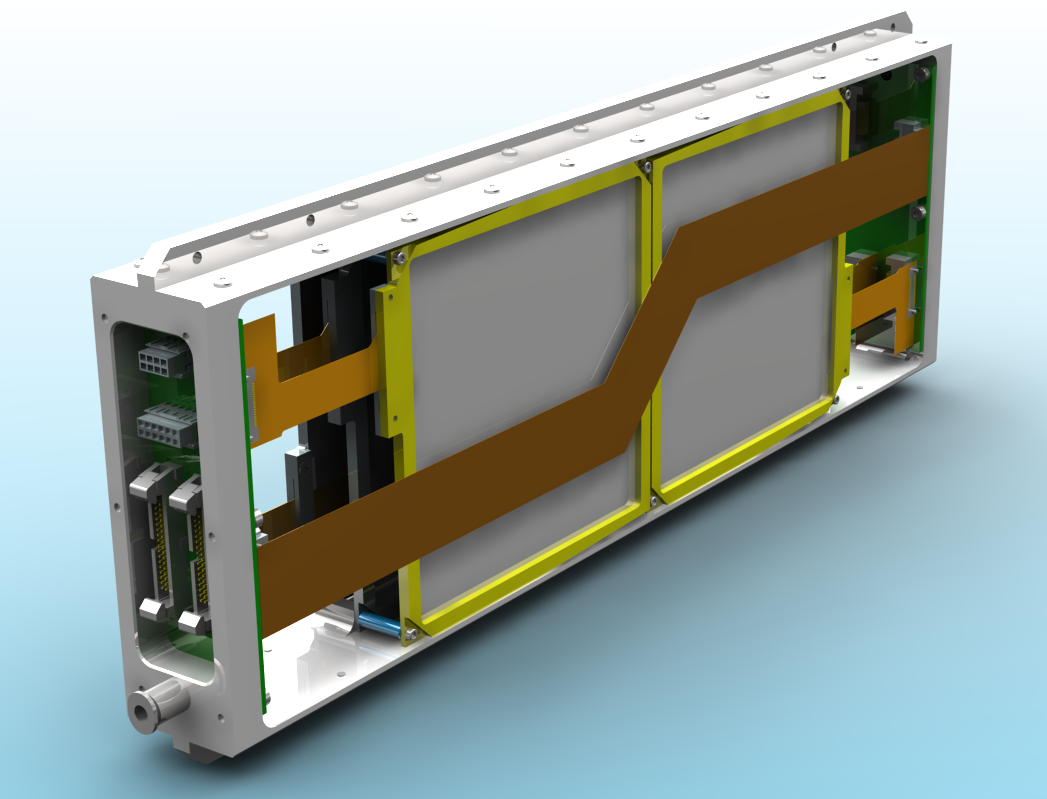
\includegraphics[width=0.33\linewidth]{pics/Si-TrackerHD}
\caption{
Left: photo of an assembled sensor module with two bump-bonded KPiX chips and a wirebonded readout kapton-flex cable glued on the sensor;
Center: sketch of the \lycoris telescope, where the black lines symbolize the module connection;
Right: 3-D drawing of the telescope holding cassette box.
}%
\label{fig:1figs}%
\end{figure}

\subsection*{Sensor module}
The SiD sensor is readout by two bump-bonded KPiX~\cite{kpix} ASICs,
each digitizes and serializes signals from 920 strips, then sends out through one single data line.
Therefore the sensor adopts a double-metal layer structure to route signals to the readout bump-bonding arrays,
and the traces on the second metal layer connect the KPiX power and signal lines to a wirebonded readout kapton cable.
This hybrid-less arrangement eliminates the material and assembly complexity of the hybrid circuit boards, that host the readout electronics.
Moreover, The KPiX chip employs a power cycle design, which lowers the power dissipation,
and thus making the gas cooling feasible to further reduce the material.
These key features enable \lycoris to host 3 sensor layers with its readout in a \SI{3.2}{\centi\metre} thick holding cassette box, see Fig.~\ref{fig:1figs}(right).

\subsubsection*{Sensor performance}
The sensors were produced by Hamamatsu, all showing very good electric features, i.e. few hundreds leakage current and all depleting at around \SI{50}{\volt}.
The assembly was done by IZM-Berlin for bump-bonding, and by DESY for cable gluing and wire-bonding.
Since this is the first time of assembling and applying this sensor,
the assembly process was carefully controlled via various tests,
including electric property tests, radioactive source ($^{90}$Sr) tests, and beam tests.

The commissioning tests on the assembled sensor modules shows the following qualities:
1) leakage current kept lower than \SI{1}{\micro\ampere};
2) a good Landau response to the incident particle;
3) a good signal to noise ratio;
Furthermore, the effect of the instantaneous currents from the KPiX power line on the second metal layer of the sensor,
on the sensor performance is studied.

\subsection*{Telescope prototype}
The prototype will host at least 2 sensor planes in each cassette.
The beam tests will be carried out at DESY with an EUDET-type beam telescope~\cite{eudet} as reference,
first without and later on with the \SI{1}{\tesla} solenoid.

A full Geant4 based simulation software has been developped, and two of the various alternative reconstruction software were tested.
The beam tests results will be compared with the simulation to study the telescope performance, such as resolution, timing, and efficiencies.
%\subsection*{commissioning test}

\subsection*{Summary}
\lycoris beam telescope is projected to deliever in January 2019, with a Trigger Logic Unit (TLU) and a reconstruction software ready-to-use for user.

This presentation will firstly introduce the telescope with its components,
then the first characterization results from this hybrid-less sensor will be highlighted including studies on timing, signal response and efficiency.
At the end, the first beam test results of the telescope prototype will be shown with a comparison to the simulation studies.
%\lycoris telescope will be presented, with its first results and a comparison to simulation;
%the characterization of the sensor and readout system will also be included.

%The presentation will first introduce the telescope with its components,
%then characterization results of the sensor modules will be given based on the beam tests in August and September 2018.
%At the end, the first beam test results of the \lycoris telescope prototype will be shown with a comparison to the simulation.

%%----- working remark ------%%

\footnotesize
\begin{thebibliography}{1}
\bibitem{aida2020} AIDA2020 homepage \url{http://aida2020.web.cern.ch}, accessed on 2018-04-05

\bibitem{kpix} J.~Brau et al., {\em KPiX - A 1,024 channel readout ASIC for the ILC},
\textbf{in 2012 IEEE Nuclear Science Symposium and Medical Imaging Conference Record (NSS/MIC), pp. 1857–1860, Oct 2012.}.
%\bibitem{desytbf} DESY II Test Beam Facility \url{http://testbeam.desy.de}, accessed on 2018-04-05

\bibitem{desytbf} R.~Diener et al., {\em The DESY II Test Beam Facility},
\textbf{arXiv:1807.09328 [physics.ins-det]}.

\bibitem{ILC-2013TDR:det}  T.~Behnke et al.,{\em The International Linear Collider Technical Design Report - Volume 4: Detectors}
\textbf{arXiv:1306.6329 [physics.ins-det]}

\bibitem{eudet} H.~Jansen et al., {\em Performance of the EUDET-type beam telescopes},
\textbf{EPJ Tech.\ Instrum.\  {\bf 3}, no. 1, 7 (2016)}.

%\bibitem{eudaq2} Y.~Liu., {\em EUDAQ2 User Manual},
%\textbf{AIDA-2020-NOTE-2018-001}.

%\bibitem{lycoris1} U.~Kraemer et al., {\em LYCORIS - A Large Area Strip Telescope},
%\textbf{arXiv:1801.08505 [physics.ins-det]}.


\end{thebibliography}

\end{document}
